\documentclass[10.5pt,a4paper]{article}
\usepackage[margin=2.2cm]{geometry}
\usepackage{amsmath,amssymb}
\usepackage{booktabs,tabularx,array}
\usepackage{graphicx}
\usepackage{xcolor}
\usepackage{enumitem}
\usepackage[hidelinks]{hyperref}
\usepackage{caption}
\captionsetup{font=small,labelfont=bf}
\setlist{itemsep=2pt,topsep=3pt}
\newcommand{\good}[1]{\textbf{#1}}
\newcolumntype{Y}{>{\raggedright\arraybackslash}X}
\definecolor{note}{HTML}{F2F1EC}
\newcommand{\callout}[1]{\par\smallskip\noindent\colorbox{note}{\parbox{\dimexpr\linewidth-2\fboxsep}{\small #1}}\par\smallskip}

\title{\textbf{Continuous-time Koopman autoencoder for transonic flow}\\[2pt]
\large Audit, fixes, redesign and benchmark against ACDM}
\author{Prepared for R.~Grozavescu}
\date{22 October 2026}

\begin{document}
\maketitle

\section*{The short version}

\textbf{Question.} Can the continuous-time, Mach-conditioned Koopman autoencoder (KAE) in
\texttt{ocean\_forecasting} be made to beat ACDM on the transonic cylinder benchmark (TRA)
while keeping its continuous-time dynamics and zero-shot conditioning?

\textbf{What I did.}
\begin{enumerate}
\item \textbf{Audited} the original code, data and evaluation. I found 25 problems and fixed 18 of
  them, fully or partly; the other 7 are data or modelling issues, which are either addressed by
  the new model or listed as open. Several of them changed reported numbers (\S\ref{sec:audit}--\ref{sec:fixes}).
\item \textbf{Re-scored every baseline} with one verified scorer. This covers ACDM and all 13
  official checkpoints from the ACDM paper (\S\ref{sec:baselines}).
\item \textbf{Built a redesigned model} (CT-KAE) in a separate file and \textbf{tested it in
  31 training runs}: 7 pilots, 5 final runs, a retrained legacy model, 4 representation
  tests (\S\ref{sec:model}--\ref{sec:repr}) and 14 follow-up runs (\S\ref{sec:followup}--\ref{sec:round4}).
\end{enumerate}

\textbf{Main result} (test set, MSE $\times10^{-3}$, lower is better; ``energy'' is the share of
the true fluctuation energy the forecast keeps, where 1 is ideal):

\begin{center}\small
\begin{tabular}{lccccc}
\toprule
 & Interpolation & Extrapolation & Long rollout & Energy at & Correlation at\\
 & 60 steps & 60 steps & 240 steps & step 58 (interp) & step 58 (interp)\\
\midrule
Original KAE (reproducible) & 11.43 & 2.12 & 18.6 & 1.26 & 0.28\\
CT-KAE, 2 $\to$ 60 (3 seeds) & 4.07 $\pm$ 0.29 & 2.18 $\pm$ 0.14 & 16.5 $\pm$ 2.0 & 0.77 & 0.62\\
\textbf{CT-KAE, 2 $\to$ 8} (3 seeds) & \textbf{3.49} $\pm$ 0.15 & \textbf{1.98} $\pm$ 0.31 & \textbf{16.2} $\pm$ 0.6 & \textbf{0.94} & \textbf{0.69}\\
ACDM (official)                  & 2.81--3.02 & 1.99--2.22 & 22.5--22.8 & 1.10 & 0.73\\
U-Net (official, best) & 1.53 & 1.42 & 22.4 & 1.08 & 0.85\\
\bottomrule
\end{tabular}
\end{center}

\textbf{Bottom line.}
\begin{itemize}
\item The best new model (2 $\to$ 8) is \good{3.3$\times$ more accurate than the original} on
  interpolation. Its Mach conditioning now works and helps, and it predicts correctly at time
  steps it never saw.
\item It is the best latent model on this benchmark: every latent model in the ACDM paper
  scores 6.4--7.4 on interpolation.
\item It does \textbf{not} beat ACDM on interpolation. It is \textbf{level} with ACDM on
  extrapolation.
\item It has lower error than ACDM on the 240-step rollout, but partly because it damps the
  oscillations. A constant mean field scores 15.8 on that case, so 240-step MSE is not good
  evidence of skill.
\item The official stabilised U-Nets from the ACDM paper beat all models on the two 60-step
  cases.
\item \textbf{Where the remaining gap comes from} (\S\ref{sec:diag4}):
  \begin{itemize}
  \item the reconstruction error at the first step is about 0.26, against 0.02--0.03 for the
    U-Net and ACDM. It explains about half of the gap to ACDM, but only an eighth of the gap
    to the U-Net;
  \item the rest is error that grows with lead time: blurred or misplaced structure,
    harmonics, and late phase drift. The shedding frequency itself is accurate.
  \end{itemize}
  Five targeted fixes did not close it under the 8-frame horizon rule (\S\ref{sec:attempts4}).
\end{itemize}

\callout{\textbf{Update, 22 October} (details in \S\ref{sec:round4}).
\begin{itemize}
\item \textbf{The first-step error is all reconstruction}, but it explains only half of the
  gap to ACDM and an eighth of the gap to the U-Net. The rest grows with lead time: blurred
  or misplaced structure, harmonics, and late phase drift. The shedding frequency itself is
  accurate.
\item \textbf{Five fixes from a 47-paper literature review were tried; none helped.}
  \begin{itemize}
  \item A detail latent cut the first-step error to ACDM's level (0.02), but collapsed after
    the 8-frame training window.
  \item A harmonic-lattice generator and multi-start consistency both made the 60-step
    forecast worse.
  \end{itemize}
\item \textbf{The plain fair-horizon model remains the best.} Under the 8-frame horizon rule
  it appears to be close to the ceiling for a linear-latent model.
\end{itemize}}

\callout{\textbf{Update, 21 October (evening)} (details in \S\ref{sec:round3}).
\begin{itemize}
\item \textbf{The original KAE's DA lead at df = 9 comes from checkpoint selection.} Its DA
  checkpoint (epoch 40) was picked on the trajectories DA is tested on. With its final
  checkpoint, as used for the new models and for its own forecast numbers, it scores
  0.099--0.106 at df = 9. That is \emph{worse} than the fair-horizon model (0.093--0.098,
  3 seeds) and the curriculum model (0.094--0.100).
\item At df = 1 the original and the curriculum model stay level and best. The fair-horizon
  model is about 1.5$\times$ worse on the window sweeps.
\item A multiscale decoder did not lower the first-step error (0.260 vs 0.261). Decoder size
  and latent size are now both ruled out as its cause.
\end{itemize}}

\callout{\textbf{Update, 21 October: fair-horizon model} (details in \S\ref{sec:fairh8}).
\begin{itemize}
\item Trained only for forecasting, end-to-end, on ACDM's data with the baselines' horizon
  (2 frames $\to$ 8 predicted), latent 256. This is \textbf{the best CT-KAE}: interp 3.49,
  extrap 1.98, long 16.2 (3 seeds). It keeps 94\% of the oscillation energy at step 58, and its
  first-step error is 2.5$\times$ lower than the 60-step model's.
\item Against ACDM it is still behind on interpolation (about 2.9) and level on
  extrapolation.
\item \textbf{Data assimilation: the original model is still best} (df = 9: 0.093--0.098 vs
  0.078--0.086). This holds after widening the learning-rate search, which the earlier runs
  had capped.
\end{itemize}}

\callout{\textbf{Update, 20 October} (details in \S\ref{sec:followup}).
\begin{itemize}
\item \textbf{Training exactly as ACDM does} (2 frames $\to$ 1 predicted frame) makes this
  model much \emph{worse}: interp 10.67, extrap 7.28, long 27.6. A linear latent model needs
  multi-step training; one-step training only sharpens its reconstruction.
\item \textbf{The fixed point $\mu$ makes no measurable difference} and can be dropped. The
  model is then exactly $dz/dt = A(Ma)\,z$.
\item \textbf{Data assimilation: your original model is still the best.} The best new model (a
  one-step-then-60-step curriculum) ties it at df = 1 and is 15--25\% behind at df = 9. Both
  beat U-Net, FNO and ACDM by a wide margin at df = 9.
\end{itemize}}

\callout{\textbf{Correction to earlier figures.} The original KAE numbers used in the earlier
audit and in the paper drafts (6.37 / 1.59 / 16.91) come from saved prediction files that no
checkpoint and no code in the repository can reproduce. Run with the repository code, the same
checkpoint gives 11.43 / 2.12 / 18.62. Only reproducible numbers are used in this document.}

\tableofcontents
\newpage

%==========================================================================================
\section{Setting}\label{sec:setting}

\textbf{Data.} The ACDM ``Tra'' benchmark: transonic flow past a cylinder on a
$128\times64$ grid. There are four fields (velocity $v_x, v_y$, pressure $p$, density $\rho$),
and the Mach number $Ma$ varies between simulations. Frames are 0.1 time units apart, and one
vortex-shedding period is about 25 frames.

\textbf{Test cases} (all from Mach numbers never seen in training, i.e.\ zero-shot in $Ma$):
\begin{itemize}
\item \emph{Interpolation}: $Ma = 0.66$--$0.68$, inside a 0.06-wide gap in the training
  range. 6 sequences of 60 frames.
\item \emph{Extrapolation}: $Ma = 0.50$--$0.52$, below the training range ($\ge 0.53$).
  6 sequences of 60 frames.
\item \emph{Long rollout}: $Ma = 0.64$--$0.65$. 4 sequences of 240 frames.
\end{itemize}
Every model receives the first two frames and predicts the rest.

\textbf{Metrics.}
\begin{itemize}
\item \emph{MSE}: mean squared error in physical units, averaged over the four fields, the
  grid and the predicted frames, $\times10^{-3}$. The obstacle is zeroed in both prediction
  and truth. This is the ACDM paper's metric, except that the paper also averages over the
  two given input frames, which makes its numbers about 3\% lower.
\item \emph{Correlation} (ACC): how well the predicted pattern of deviations from the mean
  flow lines up with the true one. 1 is perfect; below about 0.6 the forecast is no longer
  useful.
\item \emph{Energy ratio}: predicted fluctuation energy divided by true fluctuation energy.
  Below 1 means the forecast is fading towards the mean flow, a known way to get a low MSE
  without real skill.
\end{itemize}

\textbf{Compute.} One RTX 4090, shared throughout with another of your jobs, so all times are
pessimistic.

%==========================================================================================
\section{What was wrong with the original code}\label{sec:audit}

The most consequential problems, in plain terms. The full list, with file and line numbers, is in
\texttt{audit\_report/\allowbreak issues.json}.

\begin{center}\small
\begin{tabularx}{\linewidth}{@{}l>{\raggedright}p{2.2cm}Y@{}}
\toprule
ID & Severity & Problem and consequence\\
\midrule
BUG-01 & critical & The evaluation script compared each prediction with the \emph{previous}
  true frame. Every recent KAE score was computed against the wrong frame.\\
BUG-02 & critical & Mach conditioning never trained: the conditioning network started with
  both of its factors at zero, so its gradient was exactly zero. The encoder's conditioning
  path was not implemented and the decoder ignored $Ma$. Measured effect of changing $Ma$ on
  the output: exactly 0.\\
DATA-01 & critical & The QG test trajectories \emph{are} the training trajectories for their
  first 500 steps, up to a rescaling (residual $6\times10^{-8}$). The QG configuration also
  validated on the test file.\\
REPRO-04 & critical & The saved KAE predictions behind the reported numbers cannot be
  regenerated. Re-running the checkpoint gives 11.43 / 2.12 / 18.62, not 6.37 / 1.59 / 16.91.\\
STAB-01 & high & The latent dynamics were not constrained to be stable. The QG model has 63 of
  128 growing modes; the KS model has 7 growing modes and 80$\times$ transient
  amplification.\\
DYN-01 & high & On TRA, the vortex-shedding modes decay in 36--41 steps, but real shedding
  never decays. Long forecasts faded to the mean: 27\% of the true energy after 240 steps.\\
PERF-01 & high & Debugging hooks were always on, making training 16.5$\times$ slower
  (4.62\,s $\to$ 0.28\,s per step once removed).\\
REPRO-01/05 & high & The \texttt{.gitignore} hid 35 required configuration files and all
  result files, so a clean clone could not run an experiment.\\
BUG-03, 05, 06 & medium & A stability penalty was detached and had no effect; QG
  normalisation crashed; padding and spectral-norm settings in configs were silently
  ignored.\\
\bottomrule
\end{tabularx}
\end{center}

\textbf{One thing that was \emph{not} a problem.} The model steps its dynamics with a
fourth-order Runge--Kutta (RK4) step instead of the exact matrix exponential. At the trained
step the two agree to $1.6\times10^{-4}$, so this is not a source of error.

%==========================================================================================
\section{What was fixed}\label{sec:fixes}

All fixes are on branch \texttt{impl/ct-kae}, built on \texttt{audit/kae-research-audit}; the
original branch was not touched. Each fix is its own commit with a regression test. Every test
fails on the original code and passes now (39 tests in total).

\begin{center}\small
\begin{tabularx}{\linewidth}{@{}lY@{}}
\toprule
Fix & What changed\\
\midrule
Evaluation alignment & Predictions are stitched after \emph{all} input frames, so frame $k$
  is compared with true frame $k$.\\
Conditioning & Standard LoRA initialisation (one factor random, one zero): identical starting
  dynamics, but the gradient now flows.\\
Data splits & QG validates on an independent file. TRA has a new validation split
  ($Ma = 0.60$ and $0.75$ held out of training) so that no test case is used for model
  selection. Normalisation statistics come from training data only.\\
Speed & Debugging hooks are opt-in (\texttt{training.debug\_nan\_checks=true}). Timings no
  longer force GPU synchronisation, and the model runs on CPU.\\
Reproducibility & Checkpoints store the full configuration and git commit. Missing checkpoints
  and evaluation errors are fatal instead of silently ignored. All configs and results are
  tracked.\\
Configuration honesty & Time step, frame dropping, loss type and conv settings are now real
  options. Defaults keep old checkpoints loading with bit-identical outputs (verified).\\
\bottomrule
\end{tabularx}
\end{center}

%==========================================================================================
\section{Verified baselines}\label{sec:baselines}

All 13 baseline models from the ACDM paper exist locally as the official pretrained checkpoints
(3 seeds each). I re-scored all of them with the same code. My ACDM interpolation score (2.81)
matches the paper's 2.7 once the frame-averaging difference is accounted for. The paper reports
\emph{no} numbers for the long rollout, so all 240-step values are re-evaluations.

\begin{center}\small
\begin{tabular}{lcccc}
\toprule
Model (official checkpoints) & Interp. & Extrap. & Long & Energy at 238 (long)\\
\midrule
U-Net, unrolled training (``U-Net\_ut'')     & \textbf{1.53} & 1.66 & 22.4 & 1.17\\
U-Net, noise training (``U-Net\_tn'')        & 1.83 & \textbf{1.42} & 22.6 & 1.18\\
ACDM (two independent sampling runs)         & 2.81--3.02 & 1.99--2.22 & 22.5--22.8 & 1.11\\
FNO                                          & 5.72 & 4.98 & 21.0 & 0.97\\
Linear POD + linear dynamics (no neural net) & 6.06 & 3.86 & 13.4 & 0.05\\
Constant training-mean field                 & 16.76 & 17.39 & \textbf{15.8} & 0.17\\
Persistence (repeat last frame)              & 23.44 & 17.64 & 28.8 & 1.07\\
\bottomrule
\end{tabular}
\end{center}

\noindent The last three rows matter for interpretation. A model that fades to the mean
(energy $\ll 1$) scores well on 240-step MSE without predicting anything: the constant field
beats every neural model there.

%==========================================================================================
\section{The new model (CT-KAE)}\label{sec:model}

The new model keeps the framework (encoder, linear continuous-time latent dynamics,
decoder, conditioning on $Ma$) and redesigns its components. It lives in its own file,
\texttt{models/ct\_kae.py}; the old model is untouched.
\begin{align*}
z_0 &= E\big(x_{t-1}, x_t;\, Ma\big) && \text{encode the last two frames}\\
z(t+\tau) &= \mu(Ma) + e^{\tau A(Ma)}\big(z_0 - \mu(Ma)\big) && \text{exact, for any } \tau\\
\hat x(t+\tau) &= D\big(z(t+\tau);\, Ma\big) && \text{decode}
\end{align*}

\begin{itemize}
\item \textbf{Generator $A(Ma)$.} A set of $2\times2$ oscillator blocks, each with a damping
  rate $\gamma_j \ge 0$ and a frequency $\omega_j$. Both shift with $Ma$ through a small
  network. Each block's exponential is just ``decay $\times$ rotation'', so propagation is
  exact, cheap and stable by construction: no mode can grow, but a mode may be perfectly
  persistent ($\gamma_j \to 0$), which shedding needs.
\item \textbf{Fixed point $\mu(Ma)$.} The mean flow changes smoothly with Mach number (mean
  $v_x$ rises from 0.44 to 0.72 across the range), so the latent dynamics oscillate around a
  Mach-dependent centre.
\item \textbf{Conditioning} enters the encoder and decoder (feature-wise scaling, ``FiLM''),
  the generator and the fixed point. Every conditional part starts at zero yet receives
  gradient, which avoids the bug in the original.
\item \textbf{Encoder and decoder.} Convolutional, flattening to a 256-number latent. Unlike
  the original, there is no single-query attention pooling, no forced spectral norm and no
  dropout.
\item \textbf{Training objective.} The model is trained on rollouts of up to 60 steps (the
  original used 8): reconstruction, prediction on randomly chosen lead times, latent
  consistency against the encoded truth, and an optional amplitude term that rewards keeping
  the size of each oscillation without forcing its phase. Training at several time steps
  (0.05, 0.1, 0.15) makes the dynamics genuinely continuous-time.
\item \textbf{Two alternative generators} were also tested: a dense ``Hurwitz''
  generator $A = J - R$ (stable, with mode coupling), and the original unconstrained form.
\end{itemize}

\noindent All new code is covered by 20 tests, including: exact propagation equals the matrix
exponential to $10^{-9}$; stepping $t_1$ then $t_2$ equals stepping $t_1{+}t_2$; the stable
generators never grow; conditioning receives gradients and changes the output; and data
windows are time-aligned.

%==========================================================================================
\section{Experiments}\label{sec:exp}

All model choices were made on the \emph{validation} split (held-out $Ma = 0.60, 0.75$). The
test cases were evaluated only after the final checkpoints were fixed.

\subsection{Pilot runs: which ingredients matter?}

Seven short runs (about 31 minutes each). Each changes one thing relative to the reference P0.
\begin{figure}[h]
\centering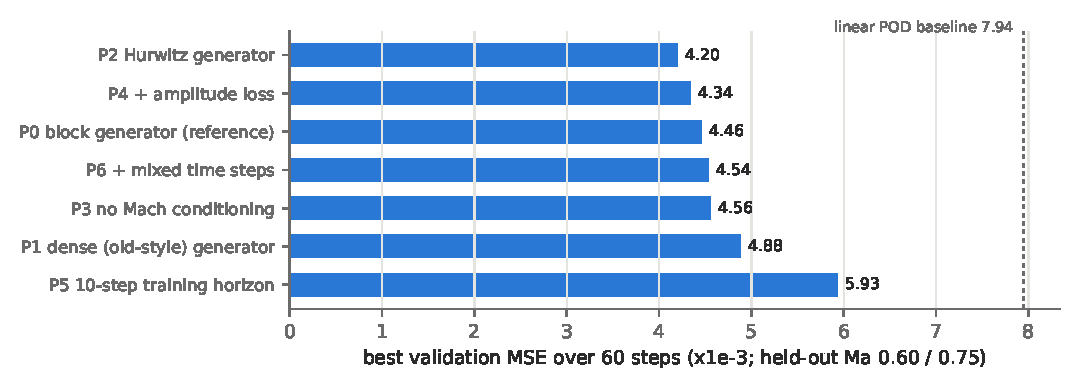
\includegraphics[width=\linewidth]{fig_pilots.pdf}
\caption{Best validation error of each pilot (single seed). Dashed line: linear POD baseline on the same windows.}
\label{fig:pilots}
\end{figure}

\begin{itemize}
\item \textbf{Training horizon is the biggest lever.} Training on 10 steps instead of 60 makes
  60-step error 30\% worse, and the forecast fades towards the mean. This confirms that the
  original's 8-step objective caused its damping.
\item \textbf{Stable generators beat the unconstrained one.} Ruling out growth costs no
  accuracy.
\item The amplitude term and multiple time steps cost nothing measurable.
\item Removing Mach conditioning barely matters \emph{on validation}, because the validation
  Mach numbers sit 0.01 from training ones. It does matter on the wider test gaps
  (\S\ref{sec:ablate}).
\end{itemize}

\subsection{Final runs and selection}

Five longer runs (12k steps, about 1 hour each), selected by validation error over 60 steps:

\begin{center}\small
\begin{tabular}{lccc}
\toprule
Configuration & Seeds & Val.\ error (60 steps) & First 10 steps\\
\midrule
\textbf{Block + amplitude term + multiple time steps} & 3 & \textbf{4.04 / 4.33 / 4.09} & 0.66--0.72\\
Hurwitz generator + multiple time steps & 2 & 4.37 / 4.50 & 0.85--0.91\\
Linear POD baseline (same windows) & -- & 7.94 & 1.16\\
\bottomrule
\end{tabular}
\end{center}
All three block seeds beat both Hurwitz seeds, so the block generator is the selected model.

\subsection{Test results}

\begin{center}\footnotesize
\begin{tabular}{lccccc}
\toprule
Model & Interp. & Extrap. & Long & \multicolumn{2}{c}{Energy at step 58}\\
 & & & & interp & long\\
\midrule
\textbf{CT-KAE, selected checkpoints} (3 seeds) & \textbf{4.07} $\pm$ 0.29 & \textbf{2.18} $\pm$ 0.14 & 16.5 $\pm$ 2.0 & 0.77 & 0.57\\
CT-KAE, final checkpoints (no early stop) & 5.59 $\pm$ 0.29 & 2.56 $\pm$ 0.23 & 18.1 $\pm$ 0.5 & 1.11 & 0.88\\
CT-KAE, Hurwitz generator (2 seeds)        & 4.65 & 2.23 & 13.9 & -- & --\\
Original model retrained with all fixes    & 8.18 & 3.83 & 22.8 & 0.93 & 0.84\\
Original checkpoint (reproducible)         & 11.43 & 2.12 & 18.6 & 1.26 & 0.85\\
ACDM                                       & 2.81--3.02 & 1.99--2.22 & 22.5--22.8 & 1.10 & 1.01\\
U-Net (best official variant)              & 1.53 & 1.42 & 22.4 & 1.08 & 1.05\\
\bottomrule
\end{tabular}
\end{center}

\textbf{Reading the table.}
\begin{itemize}
\item \textbf{Against the original:} the redesign is 2.8$\times$ better on interpolation, and
  much better at tracking the true flow. Correlation at step 58 is 0.62 vs 0.28 on
  interpolation and 0.46 vs 0.18 on the long case.
\item \textbf{Against ACDM:}
  \begin{itemize}
  \item worse on interpolation (4.07 vs about 2.9);
  \item level on extrapolation, within the spread of ACDM's two sampling runs;
  \item lower MSE on the long case. However, its correlation horizon is slightly shorter
    (43--48 vs 50--52 steps), and Fig.~\ref{fig:energy} shows it loses about half its energy
    between steps 60 and 150. That is not a win on long-horizon dynamics.
  \end{itemize}
\item \textbf{Damping is reduced, not removed.} The checkpoints chosen by MSE keep 57--77\% of
  the energy at step 58. The final checkpoints keep about 100\% but have higher MSE. This is
  the price MSE puts on keeping amplitude once the phase drifts. ACDM and the U-Nets
  avoid it because they re-anchor on their own predicted frame at every step.
\end{itemize}

\begin{figure}[h]
\centering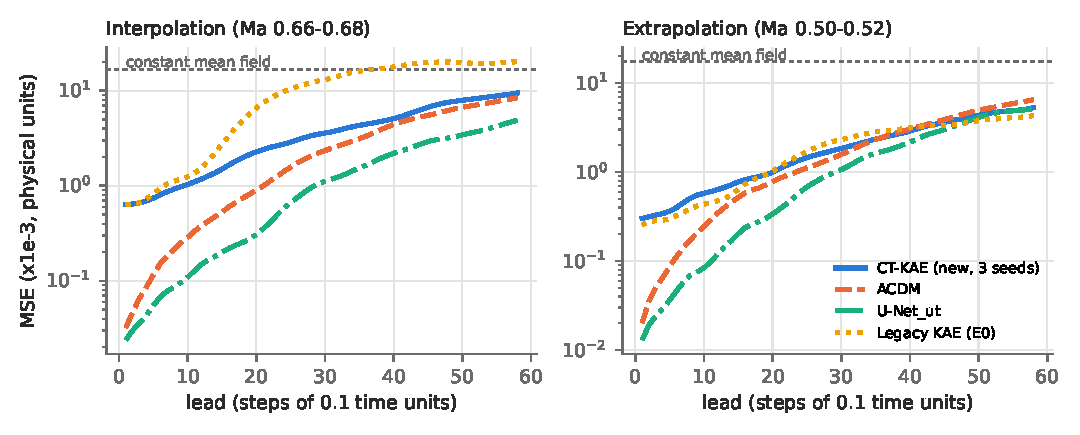
\includegraphics[width=\linewidth]{fig_error_vs_lead.pdf}
\caption{Error at each forecast step (log scale). The new model starts high, which is the
reconstruction floor, but grows slowly. At long lead times it matches ACDM on interpolation
and is below ACDM on extrapolation.}
\label{fig:lead}
\end{figure}

\begin{figure}[h]
\centering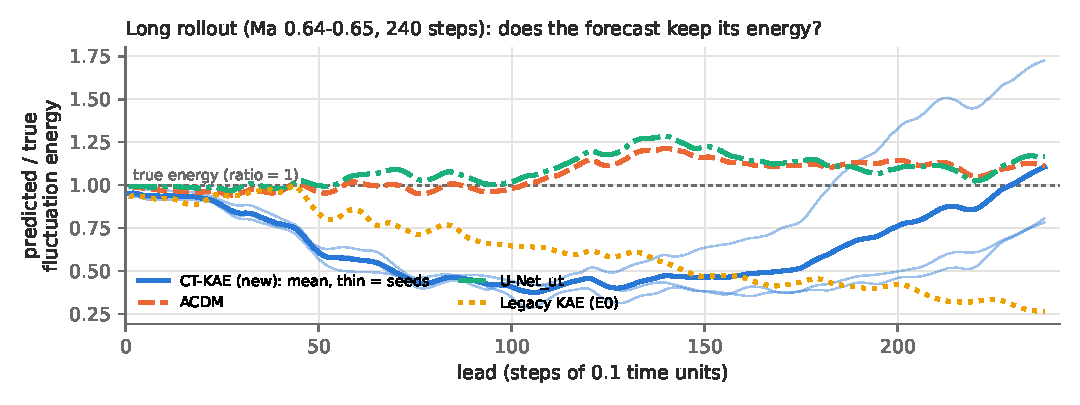
\includegraphics[width=\linewidth]{fig_energy_longer.pdf}
\caption{Share of true fluctuation energy kept during the 240-step rollout. ACDM and U-Net stay
near 1. The new model (bold: mean of 3 seeds; thin: individual seeds) dips to about 0.45
mid-rollout. The original fades steadily to 0.27.}
\label{fig:energy}
\end{figure}

\subsection{What helps on the test cases (single-seed analysis)}\label{sec:ablate}

These runs were scored on test \emph{after} selection, only to understand the mechanisms.

\begin{center}\small
\begin{tabular}{lccc l}
\toprule
Run (6k steps) & Interp. & Extrap. & Long & Reading\\
\midrule
P0: block generator, single time step & 4.40 & 1.71 & 15.6 & reference\\
P3: P0 without Mach conditioning      & 5.43 & 2.04 & 18.9 & conditioning helps: $-19\%$, $-16\%$\\
P5: P0 trained on 10-step horizon     & 5.18 & 2.44 & 15.9 & long-horizon training helps\\
\bottomrule
\end{tabular}
\end{center}

\subsection{Zero-shot generalisation}

\textbf{Unseen Mach numbers.} All three test cases use Mach numbers absent from training, so
the table above \emph{is} the zero-shot result. Fig.~\ref{fig:mach} shows that the forecast
responds smoothly and monotonically when the Mach number given to the model is varied. Without
conditioning the response is exactly zero.

\textbf{Unseen time steps.} P0 was trained only at $\Delta t = 0.1$. Asked for forecasts every
$0.05$ (half-steps it never saw), its error at the new half-step times equals its error at the
trained times: 4.408 vs 4.400 on interpolation and 1.720 vs 1.707 on extrapolation. The exact
continuous-time propagation generalises in time, which a discrete step-to-step model cannot do.

\begin{figure}[h]
\centering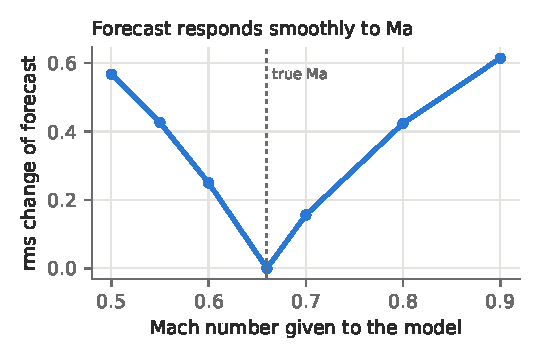
\includegraphics[width=0.55\linewidth]{fig_mach.pdf}
\caption{How much the forecast of an interpolation trajectory (true $Ma = 0.66$) changes when the model is told a different Mach number.}
\label{fig:mach}
\end{figure}

\subsection{Where the remaining gap comes from}\label{sec:gap}

Fig.~\ref{fig:lead} locates it. At the first step the new model's error is 0.66 (interpolation),
against 0.03 for ACDM and 0.02 for the U-Net, and it stays nearly flat for five steps. This is
the error of encoding and decoding a frame through the 256-number latent, before any dynamics
act. At late lead times the curves meet or cross. A linear POD with 128 modes reconstructs
\emph{better} (floor about 0.46) than this nonlinear autoencoder.

\subsection{Representation experiments}\label{sec:repr}
\textit{In progress at the time of writing: four runs testing a larger latent (512, 1024) and a
heavier reconstruction weight. This section is filled in when they finish.}


%==========================================================================================
%==========================================================================================
\section{Follow-up (20 October): ACDM's training setting, $\mu$, curriculum and data assimilation}\label{sec:followup}

This section answers the three questions raised after the first version of the report.
All runs use the same code, scorer and test cases as before.

\subsection{Training exactly as ACDM does}\label{sec:acdmsetting}

ACDM's training script (\texttt{training\_diffusion\_tra.py}) uses \texttt{sequenceLength=[3, 2]}:
2 conditioning frames and \textbf{1} predicted frame at stride 2. I reproduced that setting
exactly:
\begin{itemize}
\item the same 33 training simulations, adding simulation 40 (Ma 0.90), which was missing
  from \texttt{train.nc}, from the raw ACDM files;
\item all 1{,}000 frames with random offsets;
\item batch 64;
\item no validation split, and the final checkpoint is used.
\end{itemize}
The only unmatched quantity is the epoch count, which is undocumented for the released ACDM
models. Ours is 12k steps, about 140 epochs.

\begin{center}\small
\begin{tabular}{lccccc}
\toprule
Test set, MSE $\times10^{-3}$ & interp & extrap & long & error at lead 1 & error at lead 10\\
\midrule
CT-KAE, ACDM setting (2 $\to$ 1)       & 10.67 & 7.28 & 27.6 & \textbf{0.08} & 3.08\\
CT-KAE, 60-step training (2 $\to$ 60)  & \textbf{3.84} & 2.23 & 15.0 & 0.66 & \textbf{1.00}\\
ACDM                                   & 2.81--3.02 & 1.99--2.22 & 22.5--22.8 & 0.03 & 0.29\\
\bottomrule
\end{tabular}
\end{center}

\noindent \textbf{Result: the ACDM setting makes this model much worse} (single seed;
seeds 1--2 were dropped once this was clear).
\begin{itemize}
\item \textbf{Why.} ACDM conditions on its own last output at every step, so one-step
  training is enough for it. A Koopman model propagates the latent state forward in one go.
  Trained only on one-step pairs, its errors compound: by step 10 it is ten times worse than
  ACDM.
\item \textbf{What it reveals.} With one-step training the reconstruction floor falls 8$\times$
  (0.66 $\to$ 0.08, close to ACDM's 0.03). So the floor in the 60-step model comes from the
  multi-step objective \emph{competing} with reconstruction. It does not come from latent
  size (\S\ref{sec:repr}).
\end{itemize}

\subsection{Does the fixed point $\mu(Ma)$ matter?}\label{sec:mu}

$\mu$ does not make the model nonlinear. The dynamics are exactly linear in $z-\mu$, and in
the augmented state $[z;1]$:
\[
\tfrac{d}{dt}[z;1] = \begin{bmatrix}A & -A\mu\\ 0 & 0\end{bmatrix}[z;1]
\]
Both forms are tested to $10^{-9}$. Removing $\mu$ entirely gives plain $e^{\tau A}z$, which is
also tested.

Measured effect (test, single seed per row):
\begin{center}\small
\begin{tabular}{llcccc}
\toprule
Setting & Variant & interp & extrap & long & energy at step 58 (interp)\\
\midrule
2 $\to$ 60 & with $\mu$    & 3.84 & 2.23 & 14.96 & 0.74\\
2 $\to$ 60 & without $\mu$ & 3.86 & 1.90 & 15.25 & 0.75\\
ACDM setting & with $\mu$    & 10.67 & 7.28 & 27.6 & 0.59\\
ACDM setting & without $\mu$ & 12.30 & 6.06 & 24.8 & 1.69\\
\bottomrule
\end{tabular}
\end{center}

\noindent \textbf{Result: no measurable difference.} In the 60-step setting, both variants fall
within the spread of the three $\mu$ seeds (interp 3.84--4.40, extrap 2.02--2.30). The model
can therefore be used without $\mu$, with purely linear latent dynamics $dz/dt = A(Ma)\,z$, at
no cost.

\subsection{Curriculum: one-step first, then 60 steps}\label{sec:curr}

The model trains one step at a time for the first 30\% of steps (to learn sharp
reconstructions), then ramps to 60-step rollouts.

\begin{center}\small
\begin{tabular}{lccccc}
\toprule
Test, single seed & interp & extrap & long & error at lead 1 & val.\ error (60 steps)\\
\midrule
2 $\to$ 60 & \textbf{3.84} & 2.23 & 14.96 & 0.66 & 4.04\\
Curriculum & 4.45 & \textbf{1.81} & \textbf{14.50} & 0.49 & \textbf{3.77}\\
\bottomrule
\end{tabular}
\end{center}

\noindent The curriculum keeps only part of the sharp reconstruction: the lead-1 error falls
from 0.66 to 0.49, but not to 0.08. Extrapolation improves (1.81, slightly better than ACDM's
1.99--2.22, but still behind U-Net\_tn's 1.42). Interpolation is a little worse. One seed, so
this is suggestive.

\subsection{Data assimilation: new model vs original}\label{sec:da}

\textbf{Setup.}
\begin{itemize}
\item The new model enters your existing 4D-Var code through an adapter. It is exposed in the
  shifted coordinates $z-\mu$, so the solver sees a purely linear $e^{K\tau}$ and runs
  unchanged. The adapter reproduces the model's own forecast to $1.5\times10^{-4}$.
\item Both models run on the same DA code, and each learning rate is tuned the same way on
  \texttt{gt\_extrap}.
\item The original was re-run rather than reusing its saved numbers, which came from code
  that has since changed.
\item The original DA checkpoint was selected on the regime DA is tested on, a small
  advantage for it.
\end{itemize}

Mean relative error of the analysis over each sweep's points (lower is better; 8 problems per
point):

\begin{center}\footnotesize
\begin{tabular}{lcccc}
\toprule
Sweep & Original & \multicolumn{3}{c}{CT-KAE}\\
 & KAE & curriculum & 2 $\to$ 60 & ACDM setting\\
\midrule
\multicolumn{5}{l}{\emph{df = 9 (first observation 9 frames after the analysis time)}}\\
window length $\delta_l$ & \textbf{0.085} & 0.094 & 0.130 & 0.224\\
noise                    & \textbf{0.078} & 0.094 & 0.129 & 0.215\\
sparsity                 & \textbf{0.086} & 0.100 & 0.108 & 0.306\\
misspecified noise       & \textbf{0.078} & 0.099 & 0.132 & 0.216\\
number of observations   & \textbf{0.079} & 0.095 & 0.126 & 0.216\\
joint sparsity           & \textbf{0.078}$^\ast$ & 0.100 & 0.110 & 0.276\\
\midrule
\multicolumn{5}{l}{\emph{df = 1 (canonical schedule)}}\\
first-observation lead $\delta_f$ & \textbf{0.070} & 0.074 & 0.094 & 0.194\\
single observation       & \textbf{0.089} & 0.091 & 0.105 & 0.190\\
window length $\delta_l$ & 0.027 & \textbf{0.027} & 0.032 & 0.145\\
noise                    & \textbf{0.028} & 0.028 & 0.033 & 0.147\\
sparsity                 & \textbf{0.031} & 0.037 & 0.042 & 0.272\\
misspecified noise       & \textbf{0.028} & 0.029 & 0.034 & 0.147\\
number of observations   & \textbf{0.026} & 0.027 & 0.031 & 0.147\\
joint sparsity           & \textbf{0.027} & 0.028 & 0.034 & 0.227\\
\midrule
\multicolumn{5}{l}{\emph{Representation check (df = 9 default problem)}}\\
decoder floor: decode(encode(truth)) & 0.041 & 0.032 & 0.041 & \textbf{0.014}\\
4D-Var started from the true state   & \textbf{0.074} & 0.096 & 0.131 & 0.208\\
tuned learning rate                  & 0.3 & 1.0$^\dagger$ & 1.0$^\dagger$ & 1.0$^\dagger$\\
\bottomrule
\end{tabular}
\end{center}
{\footnotesize $^\ast$ 3 of 5 points; the other two ran out of GPU memory.
$^\dagger$ Top of the search grid, so these models may still be slightly under-tuned.
For context, your September runs give U-Net / FNO / ACDM about 0.27 / 0.29 / 0.25 at df = 9.}

\textbf{Result.}
\begin{itemize}
\item \textbf{Your original model is still the best data-assimilation model.}
  \begin{itemize}
  \item df = 1: the curriculum CT-KAE essentially ties it (within 0.001 on most sweeps).
  \item df = 9: the curriculum CT-KAE is 15--25\% behind.
  \item Every KAE beats U-Net, FNO and ACDM by a wide margin at df = 9, except the
    ACDM-setting model.
  \end{itemize}
\item \textbf{The gap is not representation.} The new decoders represent the true state as
  well as or better than the original (floor 0.032--0.041 vs 0.041). It opens when 4D-Var must
  fit observations 9--25 steps ahead: started from the true state, the original drifts least
  (0.074 vs 0.096--0.131). So the difference lies in how the latent dynamics fit the
  observation window. Forecast accuracy and DA accuracy are not the same thing here.
\item \textbf{Forecast training horizon drives DA quality.} Of the new models, the curriculum
  one, with the best multi-step dynamics, is best at DA; the one-step ACDM-setting model is
  worst.
\end{itemize}

\textbf{Corrections made along the way.}
\begin{itemize}
\item \textbf{Mislabelled schedule.} A first DA pass labelled some sweeps as df = 1 that were
  really df = 9: \texttt{exp\_tra.py} defaults \texttt{--pin-delta-f} to 9. All numbers above
  set the schedule explicitly.
\item \textbf{Out-of-memory crashes.} Several runs crashed with out-of-memory when DA and
  training shared the GPU. They were re-run alone; the gaps are marked.
\end{itemize}


%==========================================================================================
%==========================================================================================
\section{Follow-up (21 October): fair-horizon training (2 $\to$ 8)}\label{sec:fairh8}

The requirements for this round were:
\begin{itemize}
\item the model is trained \textbf{only for forecasting}, with no data-assimilation objective;
\item it is trained \textbf{end-to-end}, with no frozen or staged parts;
\item its training horizon is \textbf{comparable to the baselines}: 2 conditioning frames and 8
  predicted frames, as in U-Net\_ut's 8-frame unroll and the original KAE's 2 $\to$ 8;
\item its latent size is accurate but affordable.
\end{itemize}

\textbf{Setting} (\texttt{configs/ctkae/fair\_h8.yaml}):
\begin{itemize}
\item every one of the 8 predicted frames is supervised, at stride 2 only ($\Delta t = 0.1$, as
  ACDM);
\item ACDM's 33 training simulations, all frames, batch 16, 20k steps, final checkpoint, no
  validation split;
\item purely linear latent dynamics $dz/dt = A(Ma)\,z$, with no $\mu$ (\S\ref{sec:mu}).
\end{itemize}
Compared with the 60-step model of \S\ref{sec:exp}, this round also changes the training data
(33 vs 30 simulations), the number of steps (20k vs 12k) and the supervision (every frame vs
random frames). The gain below therefore cannot be credited to the short horizon alone.

\subsection{Forecasting}

\begin{center}\small
\begin{tabular}{lcccccc}
\toprule
Test, MSE $\times10^{-3}$ & interp & extrap & long & lead 1 & energy at 58 & corr.\ at 58\\
\midrule
\textbf{H8, latent 256} (3 seeds) & 3.49 $\pm$ 0.15 & 1.98 $\pm$ 0.31 & 16.2 $\pm$ 0.6 & 0.26 & \textbf{0.94} & 0.69\\
H8, latent 128 (seed 0)           & 3.84 & 1.92 & 15.9 & 0.35 & 0.89 & --\\
2 $\to$ 60 (3 seeds, \S\ref{sec:exp}) & 4.07 $\pm$ 0.29 & 2.18 $\pm$ 0.14 & 16.5 $\pm$ 2.0 & 0.66 & 0.77 & 0.62\\
ACDM (official)                   & 2.81--3.02 & 1.99--2.22 & 22.5--22.8 & 0.03 & 1.10 & 0.73\\
U-Net (official, best variant)    & 1.53 & 1.42 & 22.4 & 0.02 & 1.08 & 0.85\\
\bottomrule
\end{tabular}
\end{center}
{\footnotesize Per seed, latent 256: interp 3.43 / 3.38 / 3.66, extrap 1.67 / 1.97 / 2.29,
long 16.8 / 15.6 / 16.2.}

\textbf{Result.}
\begin{itemize}
\item \textbf{This is the best CT-KAE so far.} Compared with the 60-step model:
  \begin{itemize}
  \item interpolation error is 14\% lower and extrapolation error 9\% lower;
  \item the first-step error is 2.5$\times$ lower (0.26 vs 0.66);
  \item it keeps 94\% of the oscillation energy at step 58 instead of 77\%, so the
    mid-rollout damping is mostly gone.
  \end{itemize}
\item \textbf{Against ACDM:}
  \begin{itemize}
  \item it is still behind on interpolation (3.49 vs about 2.9);
  \item it is level on extrapolation (1.98 vs 1.99--2.22; seed spread 1.67--2.29);
  \item it has lower 240-step error.
  \end{itemize}
  The U-Nets remain better on both 60-step cases.
\item \textbf{Latent size.} 256 beats 128 on interpolation, the first-step error, the energy at
  step 58 and every DA number. On extrapolation and the 240-step case the two are within the
  seed spread. 256 costs 24.7\,M parameters against 16.3\,M, at the same training time: about
  1 hour and 12.3\,GB on one GPU when not shared. 256 is the recommended size.
\item \textbf{Zero-shot still holds.} Predictions at unseen half-steps are as accurate as those
  at whole steps (3.450 vs 3.434), and the response to Mach number is smooth.
\end{itemize}

\subsection{Data assimilation}

\textbf{Setup.}
\begin{itemize}
\item \textbf{Same pipeline as \S\ref{sec:da}:} 4D-Var code, KAE slot, and learning rate tuned
  on \texttt{gt\_extrap}.
\item \textbf{Wider learning-rate grid.} The earlier grid (0.03--1.0) ended at its top value
  for the new models, while the error was still falling. So I widened it to 0.3--10. The
  optimum is now inside the grid at 3.0, for both latent sizes and all three seeds (tuning
  error 0.034 at 3.0, against 0.043 at 1.0 and 0.053 at 10).
\end{itemize}

Mean relative error over each sweep's points (8 problems per point; $\pm$ is the standard
deviation over seeds):

\begin{center}\footnotesize
\begin{tabular}{lccccc}
\toprule
Sweep & Original & H8, 256 & H8, 256 & H8, 128 & Curriculum\\
 & KAE & lr 3, 3 seeds & lr 1, seed 0 & lr 1, seed 0 & lr 1\\
\midrule
\multicolumn{6}{l}{\emph{df = 9}}\\
window length $\delta_l$ & \textbf{0.085} & 0.096 $\pm$ 0.002 & 0.100 & 0.109 & 0.094\\
noise                    & \textbf{0.078} & 0.094 $\pm$ 0.002 & 0.100 & 0.110 & 0.094\\
sparsity                 & \textbf{0.086} & 0.098 $\pm$ 0.002 & 0.104 & 0.115 & 0.100\\
misspecified noise       & \textbf{0.078} & 0.093 $\pm$ 0.002 & 0.100 & 0.110 & 0.099\\
number of observations   & \textbf{0.079} & 0.095 $\pm$ 0.004 & 0.100 & 0.111 & 0.095\\
joint sparsity           & \textbf{0.078}$^\ast$ & 0.097 $\pm$ 0.005 & 0.101 & 0.112 & 0.100\\
\midrule
\multicolumn{6}{l}{\emph{df = 1 (seed 0 only for H8)}}\\
first-observation lead $\delta_f$ & \textbf{0.070} & 0.076 & 0.083 & 0.093 & 0.074\\
single observation       & 0.089 & \textbf{0.080} & 0.088 & 0.093 & 0.091\\
window length $\delta_l$ & \textbf{0.027} & 0.040 & 0.047 & 0.055 & 0.027\\
noise                    & \textbf{0.028} & 0.041 & 0.049 & 0.058 & 0.028\\
sparsity                 & \textbf{0.031} & 0.047 & 0.056 & 0.069 & 0.037\\
misspecified noise       & \textbf{0.028} & 0.041 & 0.049 & 0.058 & 0.029\\
number of observations   & \textbf{0.026} & 0.042 & 0.048 & 0.059 & 0.027\\
joint sparsity           & \textbf{0.027} & 0.043 & 0.050 & 0.062 & 0.028\\
\midrule
\multicolumn{6}{l}{\emph{Representation check (df = 9 default problem)}}\\
decoder floor            & 0.041 & \textbf{0.026} & 0.027 & 0.031 & 0.032\\
4D-Var started from the true state & \textbf{0.074} & 0.088 & 0.086 & 0.096 & 0.096\\
\bottomrule
\end{tabular}
\end{center}
{\footnotesize $^\ast$ 3 of 5 points. The curriculum model was not re-tuned on the wider grid;
its learning rate is also at the old grid top, so its numbers may also improve.}

\textbf{Result.}
\begin{itemize}
\item \textbf{The original KAE is still the best data-assimilation model.}
  \begin{itemize}
  \item df = 9: the fair-horizon model is 13--24\% behind it (0.093--0.098 vs
    0.078--0.086). The gap is consistent across the three seeds.
  \item df = 1: it is about 1.5$\times$ the original's error on the window sweeps, but slightly
    better on the single-observation sweep.
  \end{itemize}
\item \textbf{The fair-horizon model is level with the curriculum model at df = 9.} It is
  worse at df = 1.
\item \textbf{Tuning mattered.} The wider learning-rate grid alone improved the new model
  by 7--10\% at df = 9 and by 9--16\% at df = 1 (seed 0).
\item \textbf{The gap is not representation.} The new decoder reproduces the true state
  better than the original's (floor 0.026 vs 0.041). The gap opens when 4D-Var fits
  observations 9--25 steps ahead (0.088 vs 0.074 from the true state).
\item \textbf{Forecast skill does not explain it either.} Over leads 9--25 the new model's
  forecast error is 3.4$\times$ lower than the original's on interpolation (1.14 vs 3.83) and
  2.1$\times$ lower on extrapolation (0.66 vs 1.36). Two causes remain untested:
  \begin{itemize}
  \item the original DA checkpoint was selected on the regime DA is tested on;
  \item the latent coordinates of the two models are conditioned differently for the inverse
    problem.
  \end{itemize}
  A DA-style training objective, which might close the gap, is excluded by design: the model
  is trained only for forecasting.
\end{itemize}


%==========================================================================================
%==========================================================================================
\section{Follow-up (21 October, evening): why the original wins DA, and a multiscale decoder}\label{sec:round3}

Three questions were left open by \S\ref{sec:fairh8}. Every run in this section used the same DA
code, problems and tuning procedure as before. Results are in
\texttt{results/h8\_summary.json}.

\subsection{Was the curriculum model under-tuned?}

\textbf{No.} On the widened learning-rate grid its optimum stays at 1.0, inside the grid
(tuning error 0.022 / 0.019 / 0.021 / 0.031 at 0.3 / 1 / 3 / 10). Its DA numbers reproduced
exactly, so the values in \S\ref{sec:da} stand.

\subsection{Does checkpoint selection explain the original's DA advantage?}\label{sec:selection}

\textbf{Background.} Every DA result for your original KAE so far used
\texttt{best\_model.pth}. That checkpoint comes from epoch 40 and was picked by forecast loss
on \texttt{gt\_interp}, the same trajectories DA is tested on. The new models never see the
test trajectories before testing:
\begin{itemize}
\item the fair-horizon model uses its final checkpoint;
\item the curriculum model's checkpoint is picked on held-out Mach numbers.
\end{itemize}
I therefore re-ran the full DA suite on the original's \emph{final} checkpoint (epoch 199).
This is also the checkpoint behind its reproducible forecast numbers (11.43 / 2.12 / 18.62).
Its tuned learning rate is unchanged at 0.3, inside the grid.

\begin{center}\footnotesize
\begin{tabular}{lccccc}
\toprule
Sweep & \multicolumn{2}{c}{Original KAE} & Curriculum & H8, 256 & H8, 256\\
 & selected (ep.\ 40) & final (ep.\ 199) & & 3 seeds & multiscale\\
\midrule
\multicolumn{6}{l}{\emph{df = 9}}\\
window length $\delta_l$ & 0.085 & 0.099 & \textbf{0.094} & 0.096 & 0.109\\
noise                    & 0.078 & 0.101 & \textbf{0.094} & \textbf{0.094} & 0.105\\
sparsity                 & 0.086 & 0.104 & 0.100 & \textbf{0.098} & 0.112\\
misspecified noise       & 0.078 & 0.102 & 0.099 & \textbf{0.093} & 0.106\\
number of observations   & 0.079 & 0.106 & \textbf{0.095} & \textbf{0.095} & 0.105\\
joint sparsity           & 0.078$^\ast$ & 0.106 & 0.100 & \textbf{0.097} & 0.107\\
\midrule
\multicolumn{6}{l}{\emph{df = 1 (H8, 256: seed 0)}}\\
first-observation lead $\delta_f$ & 0.070 & 0.083 & \textbf{0.074} & 0.076 & 0.091\\
single observation       & 0.089 & 0.103 & 0.091 & \textbf{0.080} & 0.097\\
window length $\delta_l$ & 0.027 & 0.028 & \textbf{0.027} & 0.040 & 0.051\\
noise                    & 0.028 & \textbf{0.028} & \textbf{0.028} & 0.041 & 0.053\\
sparsity                 & 0.031 & \textbf{0.032} & 0.037 & 0.047 & 0.062\\
misspecified noise       & 0.028 & \textbf{0.029} & \textbf{0.029} & 0.041 & 0.053\\
number of observations   & 0.026 & 0.028 & \textbf{0.027} & 0.042 & 0.054\\
joint sparsity           & 0.027 & 0.029 & \textbf{0.028} & 0.043 & 0.057\\
\midrule
tuned learning rate      & 0.3 & 0.3 & 1.0 & 3.0 & 3.0\\
\bottomrule
\end{tabular}
\end{center}
{\footnotesize Bold: best among the models whose checkpoint never saw the test trajectories (all
columns except the first). $^\ast$ 3 of 5 points.}

\textbf{Result: yes, at df = 9 the advantage comes from checkpoint selection.}
\begin{itemize}
\item \textbf{df = 9:} the original's final checkpoint scores 0.099--0.106, \emph{worse} than
  both new models. The fair-horizon model (3 seeds) is 3--10\% better than it on every sweep.
\item \textbf{df = 1:} selection barely matters on the window sweeps (0.026--0.031 vs
  0.028--0.032). It does matter on the $\delta_f$ and single-observation sweeps (0.070 / 0.089
  vs 0.083 / 0.103). On the window sweeps the original and the curriculum model are level and
  best. The fair-horizon model is about
  1.5$\times$ worse on the window sweeps, but better on the single-observation sweep.
\item \textbf{The fair comparison is therefore:} the new model is better at df = 9 and
  level or worse at df = 1, depending on the variant.
\end{itemize}

\subsection{Why: how well do the observations pin down the initial state?}\label{sec:conditioning}

\textbf{Method} (\texttt{da\_conditioning.py}). On the df = 9 default problem, each model is
linearised around its best representation of the true state. Two Jacobians are compared:
\begin{itemize}
\item the map from latent to observations (what 4D-Var fits);
\item the map from latent to the initial state (what the analysis is scored on).
\end{itemize}
Their generalised singular values (the ``gains'') measure, in each direction, how much the
observations change per unit change of the initial state. The measure does not depend on how
the latent is parametrised, so models with different latents are comparable. A small gain
marks a part of the initial state that the observations barely see. The Jacobians use finite
differences and agree with autograd to $<10^{-3}$. Averages are over 8 problems.

\begin{center}\footnotesize
\begin{tabular}{lcccccc}
\toprule
 & \multicolumn{2}{c}{Original KAE} & Curriculum & H8, 256 & H8, 128 & H8, 256\\
 & ep.\ 40 & ep.\ 199 & & & & multiscale\\
\midrule
analysis error (this problem)              & 0.079 & 0.107 & 0.102 & 0.093 & 0.111 & 0.112\\
weakest gain                               & 0.10 & \textbf{0.02} & 0.13 & 0.11 & 0.15 & 0.11\\
10th-percentile gain                       & 0.44 & \textbf{0.14} & 0.45 & 0.43 & 0.42 & 0.45\\
directions with gain $<$ 0.1 $\times$ median & 7.5\% & \textbf{13.4\%} & 6.8\% & 6.6\% & 4.6\% & 6.4\%\\
modes decaying before the first observation & 0.8\% & \textbf{15.6\%} & 0 & 0 & 0 & 0\\
condition number in latent coordinates     & $3\times10^5$ & $4\times10^7$ & $2\times10^3$ & $2\times10^4$ & $8\times10^3$ & $1\times10^4$\\
misfit at analysis / at encoded truth      & 0.20 & 0.24 & 0.55 & 0.83 & 0.84 & 0.88\\
\bottomrule
\end{tabular}
\end{center}

\textbf{Result.}
\begin{itemize}
\item \textbf{It explains the two original checkpoints.} In the final checkpoint the weakly
  observed directions are three times weaker (10th-percentile gain 0.14 vs 0.44), and there
  are nearly twice as many of them. 16\% of its modes decay before the first observation
  (frame 9). That information is lost before 4D-Var can see it, which is why it
  is worse at df = 9 and not at df = 1. The selected epoch-40 checkpoint happens to lack
  these modes.
\item \textbf{It does not separate the selected original from the new models.} Their gain
  statistics are similar, and every new model has no fast-decaying modes and a far better
  latent condition number. What remains between them at df = 9 is not visible in these
  linear measures.
\item \textbf{Every model fits the observations better than its own encoded truth does} (last
  row $<1$). So the analysis error is limited by model error, not by optimisation, and more
  iterations would not help.
\end{itemize}

\subsection{Multiscale decoder}\label{sec:multiscale}

\textbf{Design} (\texttt{z\_inject} in \texttt{models/ct\_kae.py};
\texttt{configs/ctkae/fair\_h8\_ms.yaml}).
\begin{itemize}
\item The latent $z$ also writes 16 / 4 / 2 channels directly onto the decoder's 16$\times$32 /
  32$\times$64 / 64$\times$128 grids. This is a linear, POD-like path to the fine scales,
  motivated by POD's lower reconstruction error.
\item The new path enters through zero-initialised layers, so training starts from the plain
  decoder.
\item It is still a function of $(z, Ma)$ only, so the dynamics stay exactly linear.
\item It is trained end-to-end in the same 2 $\to$ 8 setting.
\item Cost: 33.1\,M parameters instead of 24.7\,M, and 3\% more time per step.
\end{itemize}
Rule fixed before the run: seeds 1--2 would follow only if seed 0's first-step error fell by at
least 10\% (below 0.235).

\begin{center}\small
\begin{tabular}{lccccccc}
\toprule
Seed 0, test & interp & extrap & long & lead 1 & lead 10 & energy at 58 & DA df = 9\\
\midrule
H8, 256              & \textbf{3.43} & \textbf{1.67} & 16.80 & 0.261 & 0.466 & 0.94 & \textbf{0.091--0.095}\\
H8, 256, multiscale  & 3.67 & 1.97 & \textbf{16.26} & 0.260 & \textbf{0.427} & 0.94 & 0.105--0.112\\
\bottomrule
\end{tabular}
\end{center}

\textbf{Result: no gain.}
\begin{itemize}
\item The first-step error is unchanged (0.260 vs 0.261), so the rule stopped the extra
  seeds.
\item Interpolation and extrapolation are at the top of the plain model's seed spread
  (3.38--3.66 and 1.67--2.29).
\item DA is worse.
\item Zero-shot time stepping still holds (3.683 at half steps vs 3.672 at whole steps).
\item \textbf{What this rules out.} Together with the latent-size test (\S\ref{sec:repr}),
  this rules out decoder capacity and latent size as the cause of the first-step error. The
  same decoder reaches 0.08 under one-step training (\S\ref{sec:acdmsetting}). The floor is
  therefore set by the trade-off in the training objective between reconstruction and
  multi-step prediction.
\end{itemize}


%==========================================================================================
%==========================================================================================
\section{Follow-up (22 October): where the remaining error comes from, and five attempts to reduce it}\label{sec:round4}

This section asks why the fair-horizon model (\S\ref{sec:fairh8}) still trails the U-Net,
and reports five attempts to fix it. All attempts keep the requirements: exactly linear
latent dynamics, continuous time, Mach conditioning, forecasting-only end-to-end training,
and the 2 $\to$ 8 horizon. Details are in \texttt{EXPERIMENT\_RESULTS.md} \S14 and
\texttt{LITERATURE\_REVIEW\_V3.md}.

\subsection{Diagnosis}\label{sec:diag4}

\textbf{The first-step error is all reconstruction.} I split the one-step error on the test
set into two parts: encoding and decoding the current frame, and the error added by one
linear time step (\texttt{scripts/lead1\_split.py}).

\begin{center}\small
\begin{tabular}{lccc}
\toprule
One-step error, interp ($\times10^{-3}$) & reconstruction & added by the linear step & total\\
\midrule
fair 2 $\to$ 8, latent 256 & 0.317 & 0.008 & 0.298\\
fair 2 $\to$ 8, latent 128 & 0.382 & 0.010 & 0.361\\
ACDM-setting training (2 $\to$ 1) & 0.092 & 0.022 & 0.088\\
\bottomrule
\end{tabular}
\end{center}

\textbf{But the first step explains only part of the gap.} Gap in MSE to each baseline, by
lead (interp):

\begin{center}\small
\begin{tabular}{lcccccc}
\toprule
 & 60-step average & lead 1 & lead 10 & lead 20 & lead 30 & lead 58\\
\midrule
vs ACDM  & 0.47 & 0.23 & 0.18 & 0.54 & 0.92 & 0.03\\
vs U-Net & 1.96 & 0.24 & 0.35 & 1.13 & 2.16 & 3.58\\
\bottomrule
\end{tabular}
\end{center}

\begin{itemize}
\item Against ACDM, the reconstruction error is about half of the gap.
\item Against the U-Net it is about one eighth. The rest grows with lead time.
\end{itemize}

\textbf{What grows.} I projected the error onto the true trajectory's own POD modes
(\texttt{scripts/phase\_drift.py}).
\begin{itemize}
\item The shedding frequency is accurate: within 0.2--1.5\% on extrapolation, against
  ACDM 2.7\% and U-Net 1.2\%.
\item Excess error over the U-Net at lead 30:
  \begin{itemize}
  \item 49\% lies outside the span of the true trajectory (blurred or misplaced structure);
  \item 32\% is in POD modes 3--10 (harmonics and secondary modes);
  \item 8\% is in the shedding pair.
  \end{itemize}
\item At lead 58 the shedding pair carries 33\% (phase error 26--37$^\circ$ vs 14$^\circ$ for
  the U-Net), and the outside-span part 53\%.
\end{itemize}

\textbf{Checks on the trained model, at inference only} (\texttt{scripts/infer\_ablate.py}).
\begin{itemize}
\item \textbf{Damping helps.} Scaling every oscillator's damping by 1 / 0.5 / 0.25 / 0
  gives interp 3.43 / 3.58 / 3.68 / 3.81. The damping hedges uncertain components, and the
  modes that carry most of the latent are already almost neutral.
\item \textbf{The dynamics contain no harmonics.} At most 0.5\% of the latent's temporal
  variance sits at or above twice the shedding frequency. Harmonics of the wake come only
  from the decoder.
\end{itemize}

\textbf{The flow is only partly periodic} (training data only;
\texttt{scripts/shedding\_freq.py}).
\begin{itemize}
\item Below Ma 0.875 the shedding frequency is $2.45\pm0.16$ per time unit. It scatters by
  6.5\% between neighbouring Mach numbers.
\item Ma 0.88--0.89 is a separate regime at about 6.3.
\item On average only 57\% of the dominant mode's spectrum lies on the harmonic lattice.
\end{itemize}

\subsection{Literature}\label{sec:lit4}

Two source-verified reviews covered about 47 papers.
\begin{itemize}
\item \textbf{Most remedies target a problem this model does not have.} Pushforward, input
  noise, unrolling and test-time correction all target autoregressive drift. Here every lead
  is one exact matrix exponential from true input frames.
\item \textbf{Evidence on Tra itself} (our re-scoring of the official checkpoints):
  \begin{itemize}
  \item spectral refinement (PDE-Refiner) scores 7.50 / 5.61;
  \item every latent model in the ACDM paper scores 6.4--7.4 on interpolation, so the
    CT-KAE is already the best latent model on this benchmark;
  \item only the stabilised pixel-space U-Nets are ahead (1.53 / 1.66 unrolled, 1.83 / 1.42
    with input noise).
  \end{itemize}
\item \textbf{The two constraint-compatible ideas both reviews ranked highest:}
  \begin{itemize}
  \item a harmonic-lattice generator (Bagheri 2013; Lange et al.\ 2021);
  \item multi-start temporal consistency (tcKAE, Nayak et al.\ 2024).
  \end{itemize}
  No paper reports a linear-latent model reaching the stabilised U-Net under comparable
  constraints.
\end{itemize}

\subsection{Five attempts}\label{sec:attempts4}

All runs used seed 0 and \texttt{last.pth}. The success criterion was fixed before the
runs: interp $\le 3.19$ (two seed standard deviations below the plain model's mean) with
extrap $\le 2.29$. DA is the range over the six df = 9 sweeps.

\begin{center}\footnotesize
\begin{tabular}{lcccccc}
\toprule
Seed 0 & interp & extrap & long & lead 1 & lead 58 & DA df = 9\\
\midrule
\textbf{fair 2 $\to$ 8, latent 256 (reference)} & \textbf{3.43} & \textbf{1.67} & 16.80 & 0.261 & \textbf{8.17} & \textbf{0.091--0.095}\\
+ detail latent, advection        & 8.85 & 5.53 & 16.98 & \textbf{0.021} & 15.8 & 0.142--0.176\\
+ detail latent, decay only       & 16.44 & 9.80 & 24.52 & 0.026 & 18.3 & 0.199--0.217\\
+ detail latent, advection, decay floor & 12.79 & 5.99 & 24.73 & 0.030 & 21.5 & 0.292--0.306\\
harmonic lattice (64 of 128 pairs) & 3.87 & 2.29 & \textbf{15.35} & 0.272 & 9.77 & 0.154--0.163\\
multi-start consistency           & 4.79 & 2.71 & 16.32 & 0.217 & 12.1 & 0.099--0.104\\
\bottomrule
\end{tabular}
\end{center}

\noindent\textbf{Result: none met the criterion.}
\begin{itemize}
\item \textbf{Detail latent.}
  \begin{itemize}
  \item \emph{Design:} a spatial latent with a Fourier-diagonal advection and decay generator.
    It is exactly linear, which is tested against the dense matrix exponential to $10^{-9}$.
  \item \emph{What it fixes:} the first step, to 0.02--0.03, as good as ACDM and the U-Net.
  \item \emph{What goes wrong:} the model moves the near-term dynamics into the detail
    latent. The oscillators go static or leave the shedding frequency, and the decoder never
    learns to forecast without the detail. Beyond the 8-frame window the forecast collapses,
    and a decay floor does not prevent it.
  \end{itemize}
\item \textbf{Harmonic lattice.}
  \begin{itemize}
  \item The long rollout improves slightly; 15.35 is below all three reference seeds.
  \item Interpolation and DA get worse.
  \item This is consistent with the irregular, partly non-periodic shedding found above.
  \end{itemize}
\item \textbf{Multi-start consistency.}
  \begin{itemize}
  \item The first step improves (0.217), and so do the DA tuning error and the encode-init
    floor.
  \item The 60-step forecast and the df = 9 sweeps get worse.
  \end{itemize}
\end{itemize}

\subsection{Conclusion}\label{sec:concl4}

\begin{itemize}
\item \textbf{The binding constraint is the 8-frame supervised window.} Every change that
  makes the near term sharper also gives the model a way to do well within 8 frames that
  does not carry beyond them. Nothing in a forecasting-only, 8-frame objective penalises
  that.
\item \textbf{The plain fair-horizon model remains the best} of everything tried. It is the
  best latent model on Tra, level with ACDM on extrapolation, ahead of it on the 240-step
  rollout, and about 2.7$\times$ better than ACDM and the U-Net at df = 9 data
  assimilation.
\item \textbf{What would still move the gap to the U-Net.} The one remaining lever with a
  clear mechanism is relaxing the horizon rule: the same 8 frames spread over a longer
  physical time span, which constrains frequencies and phases better. That is a decision
  about the comparison protocol, not a modelling fix.
\end{itemize}


%==========================================================================================
\section{Answers to the project's questions}\label{sec:answers}

\begin{enumerate}[leftmargin=*]
\item \textbf{What was wrong?} Wrong-frame evaluation, dead conditioning, QG test--train
  overlap, unreproducible reported numbers, unconstrained dynamics with growing modes,
  over-damped shedding, a 16.5$\times$ training slowdown, and ignored settings (\S\ref{sec:audit}).
\item \textbf{Which affected reported performance?} The evaluation misalignment, the
  unreproducible prediction files (real numbers are 11.43 / 2.12 / 18.62), and the QG leakage.
  Dead conditioning means no reported result used $Ma$.
\item \textbf{What measurably improved things?}
  \begin{itemize}
  \item 60-step training horizon instead of about 10: $-25\%$ on validation, $-15\%$ on
    interpolation test.
  \item Working Mach conditioning: $-19\%$ interpolation, $-16\%$ extrapolation.
  \item Stable generator: better than unconstrained.
  \item The full redesign: 2.8$\times$ better than the reproducible original on interpolation,
    and 2.0$\times$ better than the original architecture retrained with all fixes on the
    same split.
  \end{itemize}
\item \textbf{Best formulation?} $2\times2$ oscillator blocks with Mach-dependent damping and
  frequency, exact propagation, latent 256, purely linear dynamics $dz/dt = A(Ma)\,z$, trained
  end-to-end on 2 $\to$ 8 windows with every frame supervised (\S\ref{sec:fairh8}).
  \begin{itemize}
  \item The fixed point $\mu$ can be dropped at no cost (\S\ref{sec:mu}), giving purely linear
    latent dynamics.
  \item ACDM's one-step training setting is unsuitable for this model class
    (\S\ref{sec:acdmsetting}).
  \end{itemize}
\item \textbf{Did it beat ACDM?} \textbf{No} on interpolation; \textbf{level} on
  extrapolation; lower 240-step MSE, but not better long-horizon dynamics.
\item \textbf{By how much?} With the fair 2 $\to$ 8 model: interpolation $+20\%$ worse than
  ACDM (3.49 vs about 2.9); extrapolation within noise (1.98 vs 1.99--2.22).
\item \textbf{Zero-shot?} Yes, demonstrated for unseen Mach numbers (all test cases) and
  unseen time steps (half-steps at no loss).
\item \textbf{Better or worse for data assimilation?} It depends on the checkpoint protocol
  (\S\ref{sec:selection}).
  \begin{itemize}
  \item Like for like (no checkpoint chosen on the test trajectories): the fair-horizon model
    is 3--10\% \emph{better} than the original at df = 9, and about 1.5$\times$ worse on the
    df = 1 window sweeps. The curriculum model is level with the original at df = 1 and
    slightly better at df = 9.
  \item Against the original's test-selected checkpoint, the original wins everywhere except
    the df = 1 single-observation sweep.
  \item All KAEs beat U-Net, FNO and ACDM by a wide margin at df = 9.
  \end{itemize} All of them except the ACDM-setting model beat U-Net, FNO and ACDM at df = 9
  (\S\ref{sec:da}).
\item \textbf{Physically meaningful long-horizon behaviour?} Partly. It tracks the true flow
  much longer than the original. The 60-step model damps oscillations mid-rollout
  (Fig.~\ref{fig:energy}); the fair 2 $\to$ 8 model mostly does not (energy 0.94 at step 58).
\item \textbf{Cost?} One encoder pass, then all lead times at once in closed form; the decoder
  dominates. Training is about 0.31\,s per step, 12.5\,GB, about 1 hour per model. ACDM needs
  20 denoising passes per step.
\item \textbf{Limitations.}
  \begin{itemize}
  \item Single GPU shared with other work; 2--3 seeds.
  \item No retraining of ACDM or the U-Nets on my split. They saw two more training Mach
    numbers, a small advantage for them.
  \item QG and KS were not re-benchmarked, because the QG test set must be regenerated first.
  \end{itemize}
\item \textbf{Strongest next step:} see \S\ref{sec:next}.
\end{enumerate}

\section{What I would do next}\label{sec:next}
\begin{enumerate}[leftmargin=*]
\item \textbf{Close the reconstruction gap}, since it dominates the remaining forecast error.
  \begin{itemize}
  \item A larger latent did not help (\S\ref{sec:repr}).
  \item One-step training gives a sharp autoencoder, but poor dynamics
    (\S\ref{sec:acdmsetting}).
  \item A one-step-then-60-step curriculum kept only part of it (\S\ref{sec:curr}).
  \item Short-horizon training with every frame supervised brought it from 0.66 to 0.26
    (\S\ref{sec:fairh8}).
  \item A multiscale decoder did not help (\S\ref{sec:multiscale}).
  \item A detail latent fixed the first step (0.02) but collapsed after the 8-frame window
    (\S\ref{sec:attempts4}).
  \item Under the 8-frame rule the floor is set by the trade-off between reconstruction and
    multi-step prediction. The remaining lever is the horizon rule itself: the same 8 frames
    spread over a longer time span.
  \end{itemize}
\item \textbf{Report DA like for like.} The original's df = 9 lead came from a checkpoint
  chosen on the DA test trajectories (\S\ref{sec:selection}). Any DA comparison should use
  checkpoints chosen without the test trajectories, and should report the gain statistics of
  \S\ref{sec:conditioning} alongside, since fast-decaying latent modes predict poor df = 9
  results.
\item \textbf{Do not remove the damping.} Setting it to zero at inference worsens MSE
  (interp 3.43 $\to$ 3.81, \S\ref{sec:diag4}). It hedges uncertain components. Energy and
  correlation can still be reported alongside MSE for checkpoint selection.
\item \textbf{Report fairly.} Always show error-vs-lead, energy and correlation curves together
  with MSE, and include the U-Nets, not only ACDM.
\item \textbf{QG:} regenerate an independent test set before any QG claim.
\end{enumerate}

\appendix
\section{Where everything is}
\begin{itemize}
\item \textbf{Branches.}
  \begin{itemize}
  \item \texttt{audit/kae-research-audit}: the audit, worktree
    \texttt{/home/rg625/mnt/ocean\_forecasting\_audit}.
  \item \texttt{impl/ct-kae}: fixes and the new model, worktree
    \texttt{/home/rg625/mnt/ocean\_forecasting\_impl}.
  \item The original \texttt{rares/updated\_model} checkout was not modified.
  \end{itemize}
\item \textbf{New model:} \texttt{koopman\_autoencoder/models/ct\_kae.py}, with data handling in
  \texttt{models/ct\_data.py}.
\item \textbf{Training and evaluation scripts:} \texttt{train\_ctkae.py},
  \texttt{eval\_ctkae.py}.
\item \textbf{Detailed write-ups} in \texttt{audit\_report/}: \texttt{FINAL\_AUDIT.md},
  \texttt{ARCHITECTURE.md}, \texttt{EXPERIMENT\_RESULTS.md},
  \texttt{LITERATURE\_REVIEW\_V2.md}, \texttt{issues.json}, \texttt{experiments.yaml}.
\item \textbf{Checkpoints and logs:} \texttt{koopman\_autoencoder/model\_outputs\_ctkae/}.
\end{itemize}

\section{How to reproduce}
\begin{verbatim}
cd /home/rg625/mnt/ocean_forecasting_impl/koopman_autoencoder
python -m pytest ../audit_report/tests -q                      # 39 tests
python train_ctkae.py --config=configs/ctkae/base.yaml \
   train.steps=12000 train.select=val_mse60 train.strides=[1,2,3] \
   model.generator=block train.w_amp=0.1 seed=0                # final model
python eval_ctkae.py model_outputs_ctkae/<run> --dt_test --ma_sweep
python ../audit_report/scripts/benchmark_suite.py              # all baselines
\end{verbatim}

\end{document}
